
\chapter{Kronecker 积与 Vec 算子}

\section{展平}

展平（flattening）是程序员常用的操作。
用 numpy 的语言来说，我们可以写
\verb|np.ones((2,3,4)).reshape(2, 12)|，把形状为 (2,3,4) 的张量展平成形状为 (2,12) 的矩阵。
类似地，在数学记号中，$\mathrm{vec}(X)$ 通常用来表示把矩阵展平成向量。

通常这么做的主要原因，是为了绕开张量通用记号不够好用的问题。
因此，有了张量图，我们完全可以避免这种操作。
不过，看看张量图如何让展平的许多性质变得更加透明，仍然很有意思。

首先注意，展平是一个线性操作，因此可以表示成一个简单的张量。
我们用三角形表示它：
\[
   \triangleright_{i,j,k}=
\begin{tikzpicture}[baseline=-.25em]
\node[triangle] (c0) at (1.5,0) {};
\draw (c0) -- ++(-.5, .5) node[midway, above right, font=\tiny] {i};
\draw (c0) -- ++(-.5, -.5) node[midway, above left, font=\tiny] {j};
\draw[double] (c0) -- ++(.5, 0) node[midway, above, font=\tiny] {k};
\end{tikzpicture}
= [i + j n = k]
.
\]
这里 $n$ 是 $i$ 边的维度。
注意，我们用双线表示展平操作的输出。
这只是一个记法选择，用来提醒自己：输出是一束由两条边组成的边。

用这个记号可以写成
\[
   \mathrm{vec}(X)_k
   = \sum_{i,j} \triangleright_{i,j,k} X_{i,j}
   =
   \begin{tikzpicture}[baseline=-.25em]
      \node (X) at (.5,0) {X};
      \node[triangle] (c0) at (1.5,0) {};
      \draw (X) edge[bend left] (c0);
      \draw (X) edge[bend right] (c0);
      \draw[double] (c0) -- ++(.5, 0) node[midway, above, font=\tiny] {k};
   \end{tikzpicture}
   .
\]
%The basic property of $\triangleright$ is that opposing triangles cancel:
$\triangleright$ 的一些基本性质如下：
\begin{align}
   \begin{tikzpicture}[baseline=-.3em]
   \node (X) at (.5,0) {\phantom{X}};
   \node[triangle] (c0) at (1.5,0) {};
   \node[triangle, rotate=180] (c1) at (2.5,0) {};
   \node (Y) at (3.5,0) {\phantom{Y}};
   \draw (X) edge[bend left] (c0);
   \draw (X) edge[bend right] (c0);
   \draw[double] (c0) -- (c1);
   \draw (Y) edge[bend left] (c1);
   \draw (Y) edge[bend right] (c1);
   \end{tikzpicture}
   &=
   \begin{tikzpicture}[baseline=-.3em]
   \node (X) at (0,0) {\phantom{X}};
   \node (Y) at (1.5,0) {\phantom{Y}};
   \draw (X) edge[bend left] (Y);
   \draw (X) edge[bend right] (Y);
   \end{tikzpicture}
   \\
   %\text{and}
   \begin{tikzpicture}[baseline=-.3em]
   \node (X) at (.5,0) {\phantom{X}};
   \node[triangle, rotate=180] (c0) at (1.5,0) {};
   \node[triangle] (c1) at (2.5,0) {};
   \node (Y) at (3.5,0) {\phantom{Y}};
   \draw[double] (X) -- (c0);
   \draw (c0) edge[bend left] (c1);
   \draw (c0) edge[bend right] (c1);
   \draw[double] (Y) -- (c1);
   \end{tikzpicture}
   &=
   \begin{tikzpicture}[baseline=-.3em]
   \node (X) at (0,0) {\phantom{X}};
   \node (Y) at (1.5,0) {\phantom{Y}};
   \draw[double] (X) -- (Y);
   \end{tikzpicture}
   \\
%.
%\end{walign}
%It's also easy to convince oneself of the following ``mixed'' property:
%\begin{align}
   \begin{tikzpicture}[baseline=-.25em, inner sep=0pt]
      \node (F0) at (0,0) {$\sbullet$};
      \node[triangle, rotate=180, inner sep=3pt] (Fab0) at (.5,.25) {};
      \node (A) at (1,.333) {};
      \node (B) at (1,.166) {};
      \node[triangle, rotate=180, inner sep=3pt] (Fcd0) at (.5,-.25) {};
      \node (C) at (1,-.166) {};
      \node (D) at (1,-.333) {};
      \draw[double] (F0) -- ++(-.4,0);
      \draw[double] (F0) -- (Fab0);
      \draw[double] (F0) -- (Fcd0);
      \draw (Fab0) -- (A);
      \draw (Fab0) -- (B);
      \draw (Fcd0) -- (C);
      \draw (Fcd0) -- (D);
   \end{tikzpicture}
   \quad&=\quad
   \begin{tikzpicture}[baseline=-.25em, inner sep=0pt]
      \node[triangle, rotate=180, inner sep=3pt] (F0) at (0,0) {};
      \node (Fab0) at (.5,.25) {$\sbullet$};
      \node (A) at (1,.333) {};
      \node (B) at (1,.166) {};
      \node (Fcd0) at (.5,-.25) {$\sbullet$};
      \node (C) at (1,-.166) {};
      \node (D) at (1,-.333) {};
      \draw[double] (F0) -- ++(-.4,0);
      \draw (F0) -- (Fab0);
      \draw (F0) -- (Fcd0);
      \draw (Fab0) -- (A);
      \draw (Fab0) -- (C.west);
      \draw (Fcd0) -- (B.west);
      \draw (Fcd0) -- (D);
   \end{tikzpicture}
   \label{eq:flatten_mix}
%\end{align}
   \\
   \label{eq:tensor_diag}
   \begin{tikzpicture}[baseline=-.5em, inner sep=0pt]
      \node (b) at (.5,0) {$\sbullet$};
      \node[triangle, rotate=180, inner sep=3pt] (r) at (1,0) {};
      \node[triangle, inner sep=3pt] (l) at (0,0) {};
      \draw[double] (b) -- (r);
      \draw[double] (b) -- (l);
      \node[triangle, rotate=90, inner sep=3pt] (F) at (.5,-.4) {};
      \draw[double] (F) -- (b);
      \draw (F) edge[bend left] ++(.05, -.4);
      \draw (F) edge[bend right] ++(-.05, -.4);
      \draw (r) edge[bend left] ++(.4, .05);
      \draw (r) edge[bend right] ++(.4, -.05);
      \draw (l) edge[bend left] ++(-.4, -.05);
      \draw (l) edge[bend right] ++(-.4, .05);
   \end{tikzpicture}
   \quad&=\quad
   \begin{tikzpicture}[baseline=-.5em, inner sep=0pt]
      \node (b1) at (.4,.1) {$\sbullet$};
      \node (b2) at (.6,-.1) {$\sbullet$};
      \draw (b1) -- (0, .1);
      \draw (b2) -- (0, -.1);
      \draw (b1) -- (1, .1);
      \draw (b2) -- (1, -.1);
      \draw (b1) -- ++(0, -.5);
      \draw (b2) -- ++(0, -.5);
   \end{tikzpicture}
\end{align}

\section{Kronecker 积}
一个 $m\times n$ 矩阵 $A$ 与一个 $r \times q$ 矩阵 $B$ 的 Kronecker 积，是如下定义的 $mr \times nq$ 矩阵 $A \otimes B$：
\[
   \renewcommand*{\arraystretch}{1.3}
   A \otimes B = \begin{bmatrix}
      A_{1,1} B & A_{1,2} B & \cdots & A_{1,n} B \\
      A_{2,1} B & A_{2,2} B & \cdots & A_{2,n} B \\
      \vdots & \vdots & \ddots & \vdots \\
      A_{m,1} B & A_{m,2} B & \cdots & A_{m,n} B
   \end{bmatrix}
   .
\]
用指标记号也可以把它写成
$(A\otimes B)_{p(r-1)+v, q(s-1)+w} = A_{rs} B_{vw}$，但这很难读。

在张量记号中，Kronecker 积只是两个矩阵的外积，并且在“两侧”都做展平：
$A\otimes B=$
\begin{tikzpicture}[baseline=-.25em]
   \node[triangle, rotate=180] (F0) at (0,0) {};
   \node (A) at (.6,.25) {A};
   \node (B) at (.6,-.25) {B};
   \node[triangle] (F1) at (1.2,0) {};
   \draw[double] (F0) -- ++(-.4,0);
   \draw[double] (F1) -- ++(.4,0);
   \draw (F0) -- (A) -- (F1);
   \draw (F0) -- (B) -- (F1);
\end{tikzpicture}
.

Kronecker 积有如下性质：
\begin{walign}
   \tag{506}
   A \otimes (B + C) &= A \otimes B + A \otimes C
                     &
   \begin{tikzpicture}[baseline=-.25em]
      \node[triangle, rotate=180] (F0) at (0,0) {};
      \node (A) at (1,.25) {A};
      \node (B) at (1,-.25) {(B+C)};
      \node[triangle] (F1) at (2,0) {};
      \draw[double] (F0) -- ++(-.4,0);
      \draw[double] (F1) -- ++(.4,0);
      \draw (F0) -- (A) -- (F1);
      \draw (F0) -- (B) -- (F1);
   \end{tikzpicture}
                     &=
   \begin{tikzpicture}[baseline=-.25em]
      \node[triangle, rotate=180] (F0) at (0,0) {};
      \node (A) at (.6,.25) {A};
      \node (B) at (.6,-.25) {B};
      \node[triangle] (F1) at (1.2,0) {};
      \draw[double] (F0) -- ++(-.4,0);
      \draw[double] (F1) -- ++(.4,0);
      \draw (F0) -- (A) -- (F1);
      \draw (F0) -- (B) -- (F1);
   \end{tikzpicture}
                   \\&&&+
   \begin{tikzpicture}[baseline=-.25em]
      \node[triangle, rotate=180] (F0) at (0,0) {};
      \node (A) at (.6,.25) {A};
      \node (B) at (.6,-.25) {C};
      \node[triangle] (F1) at (1.2,0) {};
      \draw[double] (F0) -- ++(-.4,0);
      \draw[double] (F1) -- ++(.4,0);
      \draw (F0) -- (A) -- (F1);
      \draw (F0) -- (B) -- (F1);
   \end{tikzpicture}
   \\
   \tag{508}
   A \otimes (B \otimes C) &= (A \otimes B) \otimes C
                     &
   \begin{tikzpicture}[baseline=-.25em]
      \node[triangle, rotate=180] (F0) at (0,0) {};
      \node (A) at (1,.333) {A};
      \node[triangle] (F1) at (2,0) {};
      \node (B) at (1,0) {B};
      \node (C) at (1,-.333) {C};
      \node[triangle, rotate=180] (F2) at (.5,-.167) {};
      \node[triangle] (F3) at (1.5,-.167) {};
      \draw[triple] (F0) -- ++(-.4,0);
      \draw[triple] (F1) -- ++(.4,0);
      \draw (F0) -- (A) -- (F1);
      \draw[double] (F0) -- (F2);
      \draw[double] (F3) -- (F1);
      \draw (F2) -- (B) -- (F3);
      \draw (F2) -- (C) -- (F3);
   \end{tikzpicture}
                     &=
   \begin{tikzpicture}[baseline=-.25em]
      \node[triangle, rotate=180] (F0) at (0,0) {};
      \node (A) at (.6,.333) {A};
      \node[triangle] (F1) at (1.2,0) {};
      \node (B) at (.6,0) {B};
      \node (C) at (.6,-.333) {C};
      \draw[triple] (F0) -- ++(-.4,0);
      \draw[triple] (F1) -- ++(.4,0);
      \draw (F0) -- (A) -- (F1);
      \draw (F0) -- (B) -- (F1);
      \draw (F0) -- (C) -- (F1);
   \end{tikzpicture}
                  \\ &&&=
   \begin{tikzpicture}[baseline=-.25em]
      \node[triangle, rotate=180] (F0) at (0,0) {};
      \node (A) at (1,.333) {A};
      \node[triangle] (F1) at (2,0) {};
      \node (B) at (1,0) {B};
      \node (C) at (1,-.333) {C};
      \node[triangle, rotate=180] (F2) at (.5,.167) {};
      \node[triangle] (F3) at (1.5,.167) {};
      \draw[triple] (F0) -- ++(-.4,0);
      \draw[triple] (F1) -- ++(.4,0);
      \draw (F2) -- (A) -- (F3);
      \draw[double] (F0) -- (F2);
      \draw[double] (F3) -- (F1);
      \draw (F2) -- (B) -- (F3);
      \draw (F0) -- (C) -- (F1);
   \end{tikzpicture}
   \\
   \tag{509}
   a A \otimes b B &= a b (A \otimes B)
   &
   \begin{tikzpicture}[baseline=-.25em]
      \node[triangle, rotate=180] (F0) at (0,0) {};
      \node (A) at (.6,.25) {a A};
      \node (B) at (.6,-.25) {b B};
      \node[triangle] (F1) at (1.2,0) {};
      \draw[double] (F0) -- ++(-.4,0);
      \draw[double] (F1) -- ++(.4,0);
      \draw (F0) -- (A) -- (F1);
      \draw (F0) -- (B) -- (F1);
   \end{tikzpicture}
   &=
   \begin{tikzpicture}[baseline=-.25em]
      \node at (-.1,.4) {ab};
      \node[triangle, rotate=180] (F0) at (0,0) {};
      \node (A) at (.6,.25) {A};
      \node (B) at (.6,-.25) {B};
      \node[triangle] (F1) at (1.2,0) {};
      \draw[double] (F0) -- ++(-.4,0);
      \draw[double] (F1) -- ++(.4,0);
      \draw (F0) -- (A) -- (F1);
      \draw (F0) -- (B) -- (F1);
   \end{tikzpicture}
   \\
   \tag{510}
   (A \otimes B)^T &= A^T \otimes B^T
                   &
      \begin{tikzpicture}[baseline=-.25em]
         \node[triangle, rotate=180, minimum size=1cm] (F0) at (0,0) {};
         \node (A) at (.6,.25) {A};
         \node (B) at (.6,-.25) {B};
         \node[triangle, minimum size=1cm] (F1) at (1.2,0) {};
         \draw (F0) -- (A) -- (F1);
         \draw (F0) -- (B) -- (F1);
         \draw[double] (F0) .. controls (-1,0) and (.6,1) .. (2,0);
         \draw[double] (F1) .. controls (2.2,0) and (.6,-1) .. (-.8,0);
      \end{tikzpicture}
                   &=
      \begin{tikzpicture}[baseline=-.25em]
         \node[triangle, rotate=180, minimum size=1cm] (F0) at (-1,0) {};
         \node (A) at (0,.25) {A};
         \node (B) at (0,-.25) {B};
         \node[triangle, minimum size=1cm] (F1) at (1,0) {};
         \draw[double] (F0) -- ++(-.4,0);
         \draw[double] (F1) -- ++(.4,0);
         \draw (A.east) .. controls (1,.1) and (0,0) .. (F0);
         \draw (A.west) .. controls (-1,.5) and (0,.5) .. (F1);
         \draw (B.east) .. controls (1,-.5) and (0,-.5) .. (F0);
         \draw (B.west) .. controls (-1,-.1) and (0,0) .. (F1);
      \end{tikzpicture}
   \\
   \tag{511}
   (A \otimes B)(C \otimes D) &= AC \otimes BD
                              &
   \begin{tikzpicture}[baseline=-.25em]
      \node[triangle, rotate=180] (F0) at (0,0) {};
      \node (A) at (.6,.25) {A};
      \node (B) at (.6,-.25) {B};
      \node[triangle] (F1) at (1.2,0) {};
      \draw[double] (F0) -- ++(-.4,0);
      \draw[double] (F1) -- ++(.4,0);
      \draw (F0) -- (A) -- (F1);
      \draw (F0) -- (B) -- (F1);
      %
      \node[triangle, rotate=180] (F2) at (1.8,0) {};
      \node (C) at (2.4,.25) {C};
      \node (D) at (2.4,-.25) {D};
      \node[triangle] (F3) at (3,0) {};
      \draw (F2) -- (C) -- (F3);
      \draw (F2) -- (D) -- (F3);
      %
      \draw[double] (F1) -- (F2);
      \draw[double] (F3) -- ++(.4,0);
   \end{tikzpicture}
                              &=
   \begin{tikzpicture}[baseline=-.25em]
      \node[triangle, rotate=180] (F0) at (0,0) {};
      \node (A) at (.5,.25) {A};
      \node (B) at (.5,-.25) {B};
      \node (C) at (1.1,.25) {C};
      \node (D) at (1.1,-.25) {D};
      \node[triangle] (F1) at (1.6,0) {};
      \draw[double] (F0) -- ++(-.4,0);
      \draw[double] (F1) -- ++(.4,0);
      \draw (F0) -- (A) -- (C) -- (F1);
      \draw (F0) -- (B) -- (D) -- (F1);
   \end{tikzpicture}
   \\
   \tag{511b}
   (A \otimes I) (I \otimes B) &= A \otimes B
               &
   \begin{tikzpicture}[baseline=-.25em]
      \node[triangle, rotate=180] (F0) at (0,0) {};
      \draw[double] (F0) -- ++(-.4,0);
      \node (A) at (.6,.25) {A};
      \node[triangle] (F1) at (1.2,0) {};
      \draw (F0) -- (A) -- (F1);
      \draw (F0) edge[bend right] (F1);
      %
      \node[triangle, rotate=180] (F2) at (1.8,0) {};
      \node (D) at (2.4,-.25) {B};
      \node[triangle] (F3) at (3,0) {};
      \draw (F2) edge[bend left] (F3);
      \draw (F2) -- (D) -- (F3);
      %
      \draw[double] (F1) -- (F2);
      \draw[double] (F3) -- ++(.4,0);
   \end{tikzpicture}
                              &=
   \begin{tikzpicture}[baseline=-.25em]
      \node[triangle, rotate=180] (F0) at (0,0) {};
      \node (A) at (.6,.25) {A};
      \node (B) at (.6,-.25) {B};
      \node[triangle] (F1) at (1.2,0) {};
      \draw[double] (F0) -- ++(-.4,0);
      \draw[double] (F1) -- ++(.4,0);
      \draw (F0) -- (A) -- (F1);
      \draw (F0) -- (B) -- (F1);
   \end{tikzpicture}
   %\\
   %%\tag{512}
   %(A \otimes B)^{-1} &= A^{-1} \otimes B^{-1} \\
   \\
   \tag{515}
   \mathrm{Tr}(A \otimes B) &= \mathrm{Tr}(A) \mathrm{Tr}(B)
   &
   \hspace{-4em}
   \begin{tikzpicture}[baseline=-.25em]
      \node[triangle, rotate=180] (F0) at (0,0) {};
      \node (A) at (.6,.25) {A};
      \node (B) at (.6,-.25) {B};
      \node[triangle] (F1) at (1.2,0) {};
      \draw (F0) -- (A) -- (F1);
      \draw (F0) -- (B) -- (F1);
      \path (F0) edge [double, out=160, in=20, looseness=4] (F1);
   \end{tikzpicture}
   \hspace{-4em}
   &=
   \hspace{-4em}
   \begin{tikzpicture}[baseline=-.25em]
      \node (A) at (.6,.2) {A};
      \node (B) at (.6,-.2) {B};
      \path (A) edge [out=160, in=20, looseness=2] (A);
      \path (B) edge [out=160, in=20, looseness=11] (B);
   \end{tikzpicture}
   \hspace{-4em}
 \\&&&=
   \vspace{-4em}
   \hspace{-1em}
    \trace{A}{1}
   \hspace{-2em}
    \trace{B}{1}
   \hspace{-1em}
\end{walign}
回忆矩阵的特征分解 \eqref{eq:eigen-decomposition}，还可以得到：
\begin{walign}
   \tag{519}
   \mathrm{eig}(A \otimes B) &= \mathrm{eig}(A) \mathrm{eig}(B)
                             &&
   \begin{tikzpicture}[baseline=-.25em, inner sep=1pt]
      \node[triangle, rotate=180] (F0) at (0,0) {};
      \node (Q1) at (.6,.25) {$Q_1$};
      \node (Q2) at (.6,-.25) {$Q_2$};
      \node (b1) at (1.25,.25) {$\sbullet$};
      \node (b2) at (1.25,-.25) {$\sbullet$};
      \node (Q1i) at (2,.25) {$Q_1^{-1}$};
      \node (Q2i) at (2,-.25) {$Q_2^{-1}$};
      \node[triangle] (F1) at (2.7,0) {};
      \draw[double] (F0) -- ++(-.4,0);
      \draw[double] (F1) -- ++(.4,0);
      \draw (F0) -- (Q1) -- (b1) -- (Q1i) -- (F1);
      \draw (F0) -- (Q2) -- (b2) -- (Q2i) -- (F1);
      \draw (b1) -- ++(0, .25) node[anchor=south] {$\lambda_1$};
      \draw (b2) -- ++(0, -.25) node[anchor=north] {$\lambda_2$};
   \end{tikzpicture}
                           \\&&&=
   \begin{tikzpicture}[baseline=-.25em, inner sep=1pt]
      \node[triangle, rotate=180] (F0) at (0,0) {};
      \node (Q1) at (.55,.25) {$Q_1$};
      \node (Q2) at (.55,-.25) {$Q_2$};
      \node[triangle] (F1) at (1.1,0) {};
      \node[triangle, rotate=180] (F2) at (1.5,0) {};
      \node (b1) at (1.9,.25) {$\sbullet$};
      \node (b2) at (1.9,-.25) {$\sbullet$};
      \node[triangle] (F3) at (2.3,0) {};
      \node[triangle, rotate=180] (F4) at (2.7,0) {};
      \node (Q1i) at (3.35,.25) {$Q_1^{-1}$};
      \node (Q2i) at (3.35,-.25) {$Q_2^{-1}$};
      \node[triangle] (F5) at (4,0) {};
      \draw[double] (F0) -- ++(-.4,0);
      \draw[double] (F5) -- ++(.4,0);
      \draw (F0) -- (Q1) -- (F1);
      \draw (F1) edge[double] (F2);
      \draw (F2) -- (b1) -- (F3);
      \draw (F3) edge[double] (F4);
      \draw (F4) -- (Q1i) -- (F5);
      \draw (F0) -- (Q2) -- (F1);
      \draw (F2) -- (b2) -- (F3);
      \draw (F4) -- (Q2i) -- (F5);
      \draw (b1) -- ++(0, .25) node[anchor=south] {$\lambda_1$};
      \draw (b2) -- ++(0, -.25) node[anchor=north] {$\lambda_2$};
   \end{tikzpicture}
                           \\&&&=
   \begin{tikzpicture}[baseline=-.25em, inner sep=1pt]
      \node[triangle, rotate=180] (F0) at (0,0) {};
      \node (Q1) at (.55,.25) {$Q_1$};
      \node (Q2) at (.55,-.25) {$Q_2$};
      \node[triangle] (F1) at (1.1,0) {};
      \node (b) at (1.6,0) {$\sbullet$};
      \node[triangle, rotate=180] (F4) at (2.1,0) {};
      \node (Q1i) at (2.75,.25) {$Q_1^{-1}$};
      \node (Q2i) at (2.75,-.25) {$Q_2^{-1}$};
      \node[triangle] (F5) at (3.4,0) {};
      \draw[double] (F0) -- ++(-.4,0);
      \draw[double] (F5) -- ++(.4,0);
      \draw (F0) -- (Q1) -- (F1);
      \draw[double] (F1) -- (b) -- (F4);
      \draw (F4) -- (Q1i) -- (F5);
      \draw (F0) -- (Q2) -- (F1);
      \draw (F4) -- (Q2i) -- (F5);
      \node[triangle, below=.3em of b, rotate=90] (Fb) {};
      \draw[double] (Fb) -- (b);
      \draw (Fb) -- ++(-.1, -.25) node[anchor=north east] {$\lambda_1$};
      \draw (Fb) -- ++(.1, -.25) node[anchor=north west] {$\lambda_2$};
   \end{tikzpicture}
\end{walign}
其中最后一步来自 \eqref{eq:tensor_diag}。

% Here the last equation shows an interesting general property of $\triangleright$:
% \begin{align}
%    \begin{tikzpicture}[baseline=-.25em]
%       \node[triangle, rotate=180] (F0) at (0,0) {};
%       \node (b1) at (.4,.25) {$\sbullet$};
%       \node (b2) at (.6,-.25) {$\sbullet$};
%       \node[triangle] (F1) at (1,0) {};
%       \draw[double] (F0) -- ++(-.4,0);
%       \draw[double] (F1) -- ++(.4,0);
%       \draw (F0) -- (b1) -- (F1);
%       \draw (F0) -- (b2) -- (F1);
%       \node (M) at (.3,-.6) {M};
%       \draw (M) -- (b1);
%       \draw (M) -- (b2);
%    \end{tikzpicture}
%    =
%    \begin{tikzpicture}[baseline=-.25em]
%       \node (b) at (.5,0) {$\sbullet$};
%       \draw[double] (b) -- ++(-.4,0);
%       \draw[double] (b) -- ++(.4,0);
%       \node[triangle, rotate=90] (F) at (.5,-.5) {};
%       \draw[double] (F) -- (b);
%       \node (M) at (.5,-1.1) {M};
%       \draw (M) edge[bend left] (F);
%       \draw (M) edge[bend right] (F);
%    \end{tikzpicture}.
%    \label{eq:tensor_diag}
% \end{align}
如果考虑
$
   V =
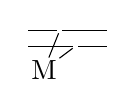
\begin{tikzpicture}[baseline=-.5em, inner sep=1pt, outer sep=0pt]
      \node (b1) at (.4,.1) {$\sbullet$};
      \node (b2) at (.6,-.1) {$\sbullet$};
      \draw (b1) -- (0, .1);
      \draw (b2) -- (0, -.1);
      \draw (b1) -- (1, .1);
      \draw (b2) -- (1, -.1);
      \node (M) at (.2,-.4) {M};
      \draw (M) -- (b1);
      \draw (M) -- (b2);
   \end{tikzpicture}
$
表示满足 $V_{i,j,i,j} = M_{i,j}$、其余分量为 0 的张量，这一点会更容易看清。
因此，对 $V$ 的两侧做展平就等同于 $\mathrm{diag}(\mathrm{vec}(M))$。


\section{Vec 算子}

Vec 算子作用在矩阵 $A$ 上时，会把各列堆叠成一个向量；也就是说，对于一个 $2\times 2$ 矩阵，
\[
   \renewcommand*{\arraystretch}{1.3}
   A = \begin{bmatrix} A_{11} & A_{12} \\ A_{21} & A_{22} \end{bmatrix}
   \quad
   \mathrm{vec}(A) = \begin{bmatrix} A_{11} \\ A_{21} \\ A_{12} \\ A_{22} \end{bmatrix}
\]

在本章开头，我们已经展示了如何用展平张量表示 Vec 算子：
$
   \mathrm{vec}(X)
   =
   \begin{tikzpicture}[baseline=-.25em]
      \node (X) at (.5,0) {X};
      \node[triangle] (c0) at (1.5,0) {};
      \draw (X) edge[bend left] (c0);
      \draw (X) edge[bend right] (c0);
      \draw[double] (c0) -- ++(.5, 0);
   \end{tikzpicture}
$.
The Matrix Cookbook 给出了 Vec 算子的如下性质：

\begin{walign}
   \tag{520}
   \mathrm{vec}(A^T X B)
   &=
   \mathrm{vec}(X)^T
   (A \otimes B)
                     &
   \begin{tikzpicture}[baseline=-.25em]
      \node (X) at (-.2,0) {X};
      \node (A) at (.5,.5) {A};
      \node (B) at (.5,-.5) {B};
      \node[triangle] (c1) at (1,0) {};
      \draw (X) -- (A) -- (c1);
      \draw (X) -- (B) -- (c1);
      \draw (c1) edge[double] ++(.5, 0);
   \end{tikzpicture}
                        &=
   \begin{tikzpicture}[baseline=-.25em]
      \node (X) at (.75,0) {X};
      \node[triangle] (c0) at (1.5,0) {};
      \node[triangle, rotate=180] (c1) at (2,0) {};
      \node (A) at (2.5,.5) {A};
      \node (B) at (2.5,-.5) {B};
      \node[triangle] (c2) at (3,0) {};
      \node (c3) at (3.4,0) {};
      \draw (X) edge[bend left] (c0);
      \draw (X) edge[bend right] (c0);
      \draw[double] (c0) -- (c1);
      \draw (c1) -- (A) -- (c2);
      \draw (c1) -- (B) -- (c2);
      \draw[double] (c2) -- (c3);
      % \draw [decorate,decoration={brace,amplitude=5pt,mirror,raise=4ex}]
      % (.5,-.75) -- (3.5,-.75) node[midway,yshift=-3em]{$\mathrm{vec}(X)^T(A \otimes B)$};
   \end{tikzpicture}
   \\
   \tag{521}
   \mathrm{Tr}(A^TB) &= \mathrm{vec}(A)^T \mathrm{vec}(B)
                     &
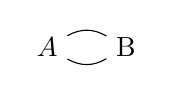
\begin{tikzpicture}[baseline=-.5em]
   \node (A) at (0,0) {$A$};
   \node (B) at (1,0) {B};
   \draw (A) edge[bend left] (B);
   \draw (A) edge[bend right] (B);
\end{tikzpicture}
&=
\begin{tikzpicture}[baseline=-.5em]
   \node (A) at (0,0) {A};
   \node (B) at (2,0) {B};
   \node[triangle] (c1) at (.66,0) {};
   \node[triangle, rotate=180] (c2) at (1.33,0) {};
   \draw (A) edge[bend left] (c1);
   \draw (A) edge[bend right] (c1);
   \draw (c1) edge[double] (c2);
   \draw (B) edge[bend left] (c2);
   \draw (B) edge[bend right] (c2);
\end{tikzpicture}
   \\
   \tag{522}
   \mathrm{vec}(A + B) &= \mathrm{vec}(A) +  \mathrm{vec}(B)
                       &
   \begin{tikzpicture}[baseline=-.25em]
      \node (a) at (0,0) {(A+B)};
      \node[triangle] (c1) at (1,0) {};
      \draw (c1) edge[double] ++(.4, 0);
      \draw (a) edge[bend left=10] (c1);
      \draw (a) edge[bend right=10] (c1);
   \end{tikzpicture}
                       &=
   \begin{tikzpicture}[baseline=-.25em]
      \node (a) at (0,0) {A};
      \node[triangle] (c1) at (.6,0) {};
      \draw (c1) edge[double] ++(.4, 0);
      \draw (a) edge[bend left=20] (c1);
      \draw (a) edge[bend right=20] (c1);
   \end{tikzpicture}
   +
   \begin{tikzpicture}[baseline=-.25em]
      \node (a) at (0,0) {B};
      \node[triangle] (c1) at (.6,0) {};
      \draw (c1) edge[double] ++(.4, 0);
      \draw (a) edge[bend left=20] (c1);
      \draw (a) edge[bend right=20] (c1);
   \end{tikzpicture}
   \\
   \tag{523}
   \mathrm{vec}(a A) &= a\, \mathrm{vec}(A)
                     &
   \begin{tikzpicture}[baseline=-.25em]
      \node (a) at (0,0) {$a A$};
      \node[triangle] (c1) at (.6,0) {};
      \draw (c1) edge[double] ++(.4, 0);
      \draw (a) edge[bend left=20] (c1);
      \draw (a) edge[bend right=20] (c1);
   \end{tikzpicture}
                     &=
   a
   \begin{tikzpicture}[baseline=-.25em]
      \node (a) at (0,0) {$A$};
      \node[triangle] (c1) at (.6,0) {};
      \draw (c1) edge[double] ++(.4, 0);
      \draw (a) edge[bend left=20] (c1);
      \draw (a) edge[bend right=20] (c1);
   \end{tikzpicture}
   \\
   \tag{524}
   a^T X B X^T c &= \mathrm{vec}(X)^T (B\otimes ca^T) \mathrm{vec}(X)
                 &
                 \vecmatvec{.5em}{a}{X,B,X}{c}
                 &=
   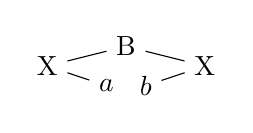
\begin{tikzpicture}[baseline=-.25em]
      \node (X1) at (2,0) {X};
      \node (B) at (3,.25) {B};
      \node (a) at (2.75,-.25) {$a$};
      \node (b) at (3.25,-.25) {$b$};
      \node (X2) at (4,0) {X};
      \draw (a) -- (X1) -- (B) -- (X2) -- (b);
   \end{tikzpicture}
               \\&&&=
   \begin{tikzpicture}[baseline=-.25em]
      \node (X) at (.75,0) {X};
      \node[triangle] (c0) at (1.5,0) {};
      \node[triangle, rotate=180] (c1) at (2,0) {};
      \node (A) at (2.75,.25) {B};
      \node (B1) at (2.5,-.25) {$a$};
      \node (B2) at (3,-.25) {$b$};
      \node[triangle] (c2) at (3.5,0) {};
      \node[triangle, rotate=180] (c3) at (4,0) {};
      \node (X1) at (4.75,0) {X};
      \draw (X) edge[bend left] (c0);
      \draw (X) edge[bend right] (c0);
      \draw (X1) edge[bend left] (c3);
      \draw (X1) edge[bend right] (c3);
      \draw[double] (c0) -- (c1);
      \draw (c1) -- (A) -- (c2);
      \draw (c1) -- (B1);
      \draw (B2) -- (c2);
      \draw[double] (c2) -- ++(.4,0);
   \end{tikzpicture}
\end{walign}

\section{Kronecker 向量积}

有时，把两个向量之间的 Kronecker 积写成矩阵会更方便。
定义
\begin{align}
   A \otimes v
   &=
   \begin{tikzpicture}[baseline=-.25em, inner sep=1pt]
      \node[triangle, rotate=180] (F0) at (0,0) {};
      \node (A) at (.5,.25) {A};
      \node (B) at (.5,-.25) {v};
      \draw[double] (F0) -- ++(-.4,0);
      \draw (F0) -- (A) -- ++(.5, 0);
      \draw (F0) -- (B);
   \end{tikzpicture}
   \label{eq:kronecker-vector}
   \\
   A \otimes v^T
   &=
   \begin{tikzpicture}[baseline=-.25em, inner sep=1pt]
      \node[triangle] (F0) at (1,0) {};
      \node (A) at (.5,.25) {A};
      \node (B) at (.5,-.25) {v};
      \draw[double] (F0) -- ++(.4,0);
      \draw (F0) -- (A) -- ++(-.5, 0);
      \draw (F0) -- (B);
   \end{tikzpicture}
   \\
   v \otimes A
   &=
   \begin{tikzpicture}[baseline=-.25em, inner sep=1pt]
      \node[triangle, rotate=180] (F0) at (0,0) {};
      \node (A) at (.5,.25) {v};
      \node (B) at (.5,-.25) {A};
      \draw[double] (F0) -- ++(-.4,0);
      \draw (F0) -- (A);
      \draw (F0) -- (B) -- ++(.5, 0);
   \end{tikzpicture}
   \\
   v^T \otimes A
   &=
   \begin{tikzpicture}[baseline=-.25em, inner sep=1pt]
      \node[triangle] (F0) at (1,0) {};
      \node (A) at (.5,.25) {v};
      \node (B) at (.5,-.25) {A};
      \draw[double] (F0) -- ++(.4,0);
      \draw (F0) -- (A);
      \draw (F0) -- (B) -- ++(-.5, 0);
   \end{tikzpicture}
\end{align}

类似地，我们可以定义两个向量之间的 Kronecker 积：
\begin{align}
   v \otimes w
   &=
   \begin{tikzpicture}[baseline=-.25em, inner sep=1pt]
      \node[triangle, rotate=180] (F0) at (0,0) {};
      \node (A) at (.5,.25) {v};
      \node (B) at (.5,-.25) {w};
      \draw[double] (F0) -- ++(-.4,0);
      \draw (F0) -- (A);
      \draw (F0) -- (B);
   \end{tikzpicture}
   \\
   v^T \otimes w^T
   &=
   \begin{tikzpicture}[baseline=-.25em, inner sep=1pt]
      \node[triangle] (F0) at (1,0) {};
      \node (A) at (.5,.25) {v};
      \node (B) at (.5,-.25) {w};
      \draw[double] (F0) -- ++(.4,0);
      \draw (F0) -- (A);
      \draw (F0) -- (B);
   \end{tikzpicture}
\end{align}

% TODO: Which of the identities 506-515 hold for the Kronecker product of vectors?

\section{一般矩阵化}

最后一个方程体现了一个一般思想：
对所有张量应用 Vec 算子、对所有边应用展平张量，就可以把任意张量网络转换成一串矩阵乘法。
例如，下面这个复杂的图：
\begin{center}
   \def\svgwidth{.7\linewidth}
   \import{figures/}{kron.pdf_tex}
\end{center}
可以写成一个简单的向量-矩阵-矩阵-向量乘积 $a M_1 M_2 b$，
其中 $M_1 = \mathrm{vec}(B) \otimes C'$，
$M_2 = E' \otimes D' \otimes I$ 且 $b = f\otimes g\otimes \mathrm{vec}(H)$。
这里 $C'$、$D'$ 和 $E'$ 是在一侧展平的三阶张量，而 $\mathrm{vec}(B)$ 被解释为只有一列的矩阵。


\subsection{Lyapunov 方程}

Kronecker 积重写的一个漂亮应用，是求解如下方程：
\begin{walign}
   \tag{272}
   AX + XB = C.
\end{walign}
我们使用重写
$
   \mathrm{vec}(AX + XB)
   =
   (I \otimes A + B^T \otimes I)\mathrm{vec}(X)
$,
它来自如下张量图变形：
\[
\begin{tikzpicture}[baseline=-.25em]
   \node at (-1,0) {$\bigg($};
   \node at (-.75,0) {$+$};
   \node (A) at (0,.25) {A};
   \node (X1) at (.75,.25) {X};
   \node (X2) at (0,-.25) {X};
   \node (B) at (.75,-.25) {B};
   \node (br) at (1.5,0) {$\bigg)$};
   \draw (A) -- (X1) -- ++(.5,0);
   \draw (A) -- ++(-.5,0);
   \draw (X2) -- (B) -- ++(.5,0);
   \draw (X2) -- ++(-.5,0);
   \node[triangle] (f) at (2.2,0) {};
   \draw (br) edge[bend right] (f);
   \draw (br) edge[bend left] (f);
   \draw[double] (f) -- ++(.4,0);
\end{tikzpicture}
=
\begin{tikzpicture}[baseline=-.25em]
   \node (X) at (0,0) {X};
   \node (B) at (.65,.25) {A};
   \node[triangle] (f) at (1.1,0) {};
   \draw (X) edge[bend right] (f);
   \draw (X) -- (B) -- (f);
   \draw[double] (f) -- ++(.4,0);
\end{tikzpicture}
+
\begin{tikzpicture}[baseline=-.25em]
   \node (X) at (0,0) {X};
   \node (A) at (.65,-.25) {B};
   \node[triangle] (f) at (1.1,0) {};
   \draw (X) edge[bend left] (f);
   \draw (X) -- (A) -- (f);
   \draw[double] (f) -- ++(.4,0);
\end{tikzpicture}
=
   \begin{tikzpicture}[baseline=-.25em]
      \node (X) at (.75,0) {X};
      \node[triangle] (c0) at (1.5,0) {};
      \draw (X) edge[bend left] (c0);
      \draw (X) edge[bend right] (c0);
      \node (bl) at (2,0) {$\bigg($};
      \node at (2.25,0) {$+$};
      \draw[double, shorten <=-4pt] (bl) -- (c0);
      \node[triangle, rotate=180] (c1) at (3,.25) {};
      \node[triangle, rotate=180] (c2) at (3,-.25) {};
      \draw[double] (c1) -- ++(-.4,0);
      \draw[double] (c2) -- ++(-.4,0);
      \node (A) at (3.4,.4) {A};
      \node (B) at (3.4,-.4) {B};
      \node[triangle] (c3) at (3.8,.25) {};
      \node[triangle] (c4) at (3.8,-.25) {};
      \draw (c1) -- (A) -- (c3);
      \draw (c2) -- (B) -- (c4);
      \draw (c1) edge[bend right] (c3);
      \draw (c2) edge[bend left] (c4);
      \draw[double] (c3) -- ++(.4,0);
      \draw[double] (c4) -- ++(.4,0);
      \node (br) at (4.4,0) {$\bigg)$};
      \draw[double, shorten <=-6pt] (br) -- ++(.2,0);
   \end{tikzpicture}
\]
之后取通常意义下的矩阵逆，就得到
\begin{walign}
   \tag{273}
   \mathrm{vec}(X) = (I \otimes A + B^T \otimes I)^{-1}\mathrm{vec}(C).
\end{walign}

\subsection{封装求和}
这是前一个方程的推广。
\begin{walign}
   \tag{274}
   \sum_n A_nXB_n &= C \\
   \tag{275}
   \mathrm{vec}(X) &= (\sum_n B_n^T \otimes A_n)^{-1} \mathrm{vec}(C)
\end{walign}

\section{Hadamard 积}
\label{sec:hadamard}

Hadamard 积也称为逐元素乘法，The Matrix Cookbook 中没有介绍它。
不过，它是一个非常有用的操作，并且有一些与 Kronecker 积相关的有趣性质。

两个 $2\times 2$ 矩阵 $A$ 和 $B$ 的 Hadamard 积定义为
\[
   \renewcommand*{\arraystretch}{1.3}
   A \circ B = \begin{bmatrix} A_{11} & A_{12} \\ A_{21} & A_{22} \end{bmatrix} \circ
              \begin{bmatrix} B_{11} & B_{12} \\ B_{21} & B_{22} \end{bmatrix}
            = \begin{bmatrix} A_{11}B_{11} & A_{12}B_{12} \\ A_{21}B_{21} & A_{22}B_{22} \end{bmatrix}
   .
\]
在张量记号中，Hadamard 积可以用两个三阶复制张量表示：
\[
   A \circ B
   =
   \begin{tikzpicture}[baseline=-.25em]
      \node (c0) at (0,0) {$\sbullet$};
      \node (A) at (.6,.25) {A};
      \node (B) at (.6,-.25) {B};
      \node (c1) at (1.2,0) {$\sbullet$};
      \draw (c0) -- (A) -- (c1);
      \draw (c0) -- (B) -- (c1);
      \draw (c0) -- ++(-.4,0);
      \draw (c1) -- ++(.4,0);
   \end{tikzpicture}
.
\]
Hadamard 积的一些性质如下：
\begin{walign}
   x^T (A \circ B) y
   &= \mathrm{tr}(A^T D_x B D_y)
   &
   \begin{tikzpicture}[baseline=-.25em, inner sep=1pt]
      \node (c0) at (0,0) {$\sbullet$};
      \node (A) at (.6,.25) {A};
      \node (B) at (.6,-.25) {B};
      \node (c1) at (1.2,0) {$\sbullet$};
      \draw (c0) -- (A) -- (c1);
      \draw (c0) -- (B) -- (c1);
      \draw (c0) -- ++(-.4,0) node[anchor=east] {x};
      \draw (c1) -- ++(.4,0) node[anchor=west] {y};
   \end{tikzpicture}
   &=
   \hspace{-2em}
   \begin{tikzpicture}[baseline=-.25em, inner sep=1pt]
      \node (A) at (0,0) {$A^T$};
      \node (c0) at (.7,0) {$\sbullet$};
      \node (B) at (1.3,0) {B};
      \node (c1) at (1.9,0) {$\sbullet$};
      \draw (A) -- (c0) -- (B) -- (c1);
      \path (A) edge [out=160, in=20, looseness=1] (c1);
      \draw (c0) -- ++(0,-.3) node[anchor=north] {x};
      \draw (c1) -- ++(0,-.3) node[anchor=north] {y};
   \end{tikzpicture}
   \hspace{-2em}
   \\
   (A \otimes B)\circ(C \otimes D) &= (A\circ C) \otimes (B\circ D)
                                   &
   \begin{tikzpicture}[baseline=-.25em, inner sep=1pt]
      \node (F0) at (0,0) {$\sbullet$};
      \node[triangle, rotate=180] (Fab0) at (.5,.5) {};
      \node (A) at (1,.75) {A};
      \node (B) at (1,.25) {B};
      \node[triangle] (Fab1) at (1.5,.5) {};
      \node[triangle, rotate=180] (Fcd0) at (.5,-.5) {};
      \node (C) at (1,-.25) {C};
      \node (D) at (1,-.75) {D};
      \node[triangle] (Fcd1) at (1.5,-.5) {};
      \node (F1) at (2,0) {$\sbullet$};
      \draw[double] (F0) -- ++(-.4,0);
      \draw[double] (F1) -- ++(.4,0);
      \draw[double] (F0) -- (Fab0);
      \draw[double] (Fab1) -- (F1);
      \draw[double] (F0) -- (Fcd0);
      \draw[double] (Fcd1) -- (F1);
      \draw (Fab0) -- (A) -- (Fab1);
      \draw (Fab0) -- (B) -- (Fab1);
      \draw (Fcd0) -- (C) -- (Fcd1);
      \draw (Fcd0) -- (D) -- (Fcd1);
   \end{tikzpicture}
                                   &=
   \begin{tikzpicture}[baseline=-.25em, inner sep=1pt]
      \node[triangle, rotate=180] (F0) at (0,0) {};
      \node (Fab0) at (.5,.5) {$\sbullet$};
      \node (A) at (1,.75) {A};
      \node (B) at (1,.25) {B};
      \node (Fab1) at (1.5,.5) {$\sbullet$};
      \node (Fcd0) at (.5,-.5) {$\sbullet$};
      \node (C) at (1,-.25) {C};
      \node (D) at (1,-.75) {D};
      \node (Fcd1) at (1.5,-.5) {$\sbullet$};
      \node[triangle] (F1) at (2,0) {};
      \draw[double] (F0) -- ++(-.4,0);
      \draw[double] (F1) -- ++(.4,0);
      \draw (F0) -- (Fab0);
      \draw (Fab1) -- (F1);
      \draw (F0) -- (Fcd0);
      \draw (Fcd1) -- (F1);
      \draw (Fab0) -- (A) -- (Fab1);
      \draw (Fab0) -- (C.west);
      \draw (C.east) -- (Fab1);
      \draw (Fcd0) -- (B.west);
      \draw (B.east) -- (Fcd1);
      \draw (Fcd0) -- (D) -- (Fcd1);
   \end{tikzpicture}
\end{walign}
第一个方程只是对张量图做变形。
第二个方程来自 \eqref{eq:flatten_mix}。
另一种看法是，只要沿着双线追踪即可：$A$ 和 $C$ 都使用双边的“上”半部分，而 $B$ 和 $D$ 使用下半部分。


\section{Khatri-Rao 积}
它也称为按列 Kronecker、按行 Kronecker 或“Face-splitting Product”。
我们分别用符号 $\ast$ 和 $\bullet$ 表示按列与按行 Kronecker 积。
\begin{walign}
   A \ast B &=
   \renewcommand*{\arraystretch}{1.3}
   \begin{bmatrix}
      A_{11} & A_{12} \\
      A_{21} & A_{22}
   \end{bmatrix}
   \ast
   \renewcommand*{\arraystretch}{1.3}
   \begin{bmatrix}
      B_{11} & B_{12} \\
      B_{21} & B_{22}
   \end{bmatrix}
            &=
   \renewcommand*{\arraystretch}{1.3}
   \begin{bmatrix}
      A_{11} B_{11} & A_{12} B_{12} \\
      A_{11} B_{21} & A_{22} B_{22} \\
      A_{21} B_{11} & A_{22} B_{12} \\
      A_{21} B_{21} & A_{22} B_{22}
   \end{bmatrix}
   \\
   A \bullet B &= \dots
            &=
   \renewcommand*{\arraystretch}{1.3}
   \begin{bmatrix}
      A_{11}  B_{11} & A_{11} B_{12} & A_{12} B_{11} & A_{12} B_{12} \\
      A_{21}  B_{21} & A_{21} B_{22} & A_{22} B_{21} & A_{22} B_{22}
   \end{bmatrix}
\end{walign}

用张量图来说，这些积只是在乘积的一侧做展平，并在另一侧使用复制张量：
\begin{walign}
   A \ast B &=
   \begin{tikzpicture}[baseline=-.25em]
      \node[triangle, rotate=180] (c0) at (0,0) {};
      \node (A) at (.6,.25) {A};
      \node (B) at (.6,-.25) {B};
      \node (c1) at (1.2,0) {$\sbullet$};
      \draw (c0) -- (A) -- (c1);
      \draw (c0) -- (B) -- (c1);
      \draw[double] (c0) -- ++(-.4,0);
      \draw (c1) -- ++(.4,0);
   \end{tikzpicture}
   \\
   A \bullet B &=
   \begin{tikzpicture}[baseline=-.25em]
      \node (c0) at (0,0) {$\sbullet$};
      \node (A) at (.6,.25) {A};
      \node (B) at (.6,-.25) {B};
      \node[triangle] (c1) at (1.2,0) {};
      \draw (c0) -- (A) -- (c1);
      \draw (c0) -- (B) -- (c1);
      \draw (c0) -- ++(-.4,0);
      \draw[double] (c1) -- ++(.4,0);
   \end{tikzpicture}
\end{walign}
显然，二者只差一个转置。
事实上，$(A \ast B)^T = B^T \bullet A^T$ 且 $(A \bullet B)^T = B^T \ast A^T$。

存在多个“混合乘积”恒等式：
\begin{walign}
   (A \bullet B)(C \otimes D) &= (A C) \bullet (B D)
                              &
   \begin{tikzpicture}[baseline=-.25em]
      \node (c0) at (0,0) {$\sbullet$};
      \draw (c0) -- ++(-.4,0);
      \node (A) at (.6,.25) {A};
      \node (B) at (.6,-.25) {B};
      \node[triangle] (c1) at (1.2,0) {};
      \draw (c0) -- (A) -- (c1);
      \draw (c0) -- (B) -- (c1);
      \node[triangle, rotate=180] (c2) at (1.7,0) {};
      \draw[double] (c1) -- (c2);
      \node (C) at (2.3,.25) {C};
      \node (D) at (2.3,-.25) {D};
      \node[triangle] (c3) at (2.9,0) {};
      \draw (c2) -- (C) -- (c3);
      \draw (c2) -- (D) -- (c3);
      \draw[double] (c3) -- ++(.4,0);
   \end{tikzpicture}
                              &=
   \begin{tikzpicture}[baseline=-.25em]
      \node (c0) at (0,0) {$\sbullet$};
      \node (A) at (.6,.25) {A};
      \node (B) at (.6,-.25) {B};
      \node (C) at (1.2,.25) {C};
      \node (D) at (1.2,-.25) {D};
      \node[triangle] (c1) at (1.8,0) {};
      \draw (c0) -- (A) -- (C) -- (c1);
      \draw (c0) -- (B) -- (D) -- (c1);
      \draw (c0) -- ++(-.4,0);
      \draw[double] (c1) -- ++(.4,0);
   \end{tikzpicture}
   \\
   (A x) \circ (B y) &= (A \bullet C) (x \otimes y)
                     &
   \begin{tikzpicture}[baseline=-.25em]
      \node (c0) at (0,0) {$\sbullet$};
      \draw (c0) -- ++(-.4,0);
      \node (A) at (.6,.25) {A};
      \node (B) at (.6,-.25) {B};
      \node (x) at (1.2,.25) {x};
      \node (y) at (1.2,-.25) {y};
      \draw (c0) -- (A) -- (x);
      \draw (c0) -- (B) -- (y);
   \end{tikzpicture}
                     &=
   \begin{tikzpicture}[baseline=-.25em]
      \node (c0) at (0,0) {$\sbullet$};
      \draw (c0) -- ++(-.4,0);
      \node (A) at (.6,.25) {A};
      \node (B) at (.6,-.25) {B};
      \node[triangle] (c1) at (1.2,0) {};
      \draw (c0) -- (A) -- (c1);
      \draw (c0) -- (B) -- (c1);
      \node[triangle, rotate=180] (c2) at (1.7,0) {};
      \draw[double] (c1) -- (c2);
      \node (x) at (2.3,.25) {x};
      \node (y) at (2.3,-.25) {y};
      \draw (c2) -- (x);
      \draw (c2) -- (y);
   \end{tikzpicture}
\end{walign}

% \section{Tracy-Singh product}
% The Tracy-Singh product is a generalization of the Kronecker product for partitioned matrices.
% For two $2\times 2$ partitioned matrices
% \[
%    A = \begin{bmatrix} A_{11} & A_{12} \\ A_{21} & A_{22} \end{bmatrix}
%    \quad\text{and}\quad
%    B = \begin{bmatrix} B_{11} & B_{12} \\ B_{21} & B_{22} \end{bmatrix}
% \]
% the Tracy-Singh product is defined as:
% \[
%    A \boxtimes B = 
%    \begin{bmatrix}
%       A_{11} \otimes B_{11} & A_{12} \otimes B_{12} \\
%       A_{21} \otimes B_{21} & A_{22} \otimes B_{22}
%    \end{bmatrix}
% \]
% 
% In tensor diagram notation, if we represent the block structure explicitly, the Tracy-Singh product can be visualized as:
% \[
% A \boxtimes B = 
% \begin{tikzpicture}[baseline=-.25em]
%    \node[draw, thick] (A) at (0,0) {\(A\)};
%    \node[draw, thick] (B) at (0,-1.5) {\(B\)};
%    \draw[thick, orange] (-1,0.5) -- (A.north west) -- (A.south west) -- (B.north west) -- (B.south west) -- (-1,-2);
%    \draw[thick, orange] (1,0.5) -- (A.north east) -- (A.south east) -- (B.north east) -- (B.south east) -- (1,-2);
% \end{tikzpicture}
% \]
% 
% More precisely, using tensor diagrams with explicit block indicators:
% \[
% \begin{tikzpicture}[baseline=-.5em, inner sep=1pt]
%    % Left side - input
%    \node (e1) at (0,1) {$e^{(i)}$};
%    \node (e2) at (0,0.3) {$e^{(j)}$};
%    \node (A) at (1,0.65) {$A$};
%    \node (e3) at (0,-0.3) {$e^{(i)}$};
%    \node (e4) at (0,-1) {$e^{(j)}$};
%    \node (B) at (1,-0.65) {$B$};
%    
%    % Connect block selectors to matrices
%    \draw (e1) -- (A);
%    \draw (e2) -- (A);
%    \draw (e3) -- (B);
%    \draw (e4) -- (B);
%    
%    % Right side - Kronecker product
%    \node[triangle, rotate=180] (F0) at (2,0) {};
%    \draw (A) -- (F0);
%    \draw (B) -- (F0);
%    \draw[double] (F0) -- ++(.6,0);
%    
%    % Output block selectors
%    \node (eo1) at (3.2,0.3) {$e^{(i)}$};
%    \node (eo2) at (3.2,-0.3) {$e^{(j)}$};
%    \draw (eo1) -- ++(-.6,0);
%    \draw (eo2) -- ++(-.6,0);
% \end{tikzpicture}
% \]
% 
% This shows that the Tracy-Singh product performs Kronecker products between corresponding blocks (selected by the same indices $i,j$).
% 
% Compare this with the standard Kronecker product in tensor notation:
% \[
% A \otimes B = 
% \begin{tikzpicture}[baseline=-.25em]
%    \node[triangle, rotate=180] (F0) at (0,0) {};
%    \node (A) at (.6,.25) {$A$};
%    \node (B) at (.6,-.25) {$B$};
%    \node[triangle] (F1) at (1.2,0) {};
%    \draw[double] (F0) -- ++(-.4,0);
%    \draw[double] (F1) -- ++(.4,0);
%    \draw (F0) -- (A) -- (F1);
%    \draw (F0) -- (B) -- (F1);
% \end{tikzpicture}
% \]
% 
% Note that unlike the standard Kronecker product where each element of $A$ multiplies the entire matrix $B$,
% in the Tracy-Singh product, each block of $A$ is Kronecker-multiplied with the corresponding block of $B$.
% This product preserves the block structure of the matrices.
% See https://arxiv.org/pdf/1903.01366

\subsection{拼接}

如果两个张量的形状匹配，就可以沿某个轴把它们拼接起来。
一种简单做法是，分别与一个选择新轴中位置的向量取外积，然后把结果相加。
定义 $e^{(i)}$ 为长度为 $2$ 的向量，它在第 $i$ 个位置为 1，其余位置为 0。
也就是说，$e^{(0)} = [1, 0]$ 且 $e^{(1)} = [0, 1]$。
于是可以定义
\[
\mathrm{cat}_i(X, Y)
=
\begin{tikzpicture}[baseline=0em, inner sep = 1pt]
    \node (e) at (0, .4) {$e^{(0)}$};
    \node (X) at (0, 0) {$X$};
    \node[triangle, rotate=180] (F) at (-.8,.2) {};
    \draw (F) -- (e);
    \draw (F) -- (X);
    \draw[double] (F) -- ++(-0.4,0) node[midway, above, font=\tiny] {$i$};
    \draw (X) -- ++(.5,0) node[midway, below, font=\tiny] {$j$};
\end{tikzpicture}
+
\begin{tikzpicture}[baseline=0em, inner sep = 1pt]
    \node (e) at (0, .4) {$e^{(1)}$};
    \node (Y) at (0, 0) {$Y$};
    \node[triangle, rotate=180] (F) at (-.8,.2) {};
    \draw (F) -- (e);
    \draw (F) -- (Y);
    \draw[double] (F) -- ++(-0.4,0) node[midway, above, font=\tiny] {$i$};
    \draw (Y) -- ++(.5,0) node[midway, below, font=\tiny] {$j$};
\end{tikzpicture}
.
\]

对于矩阵和向量，我们常用竖线来表示拼接，例如：
$\mathrm{stack}_i(A, B) = A\mid B$ 和 $\mathrm{stack}_j(A, B) = A \mid B$。
由此得到恒等式
\begin{align*}
\left(A \mid C\right) \left(\frac{B}{D}\right)
&=
\mathrm{stack}_i(A, C)
\,
\mathrm{stack}_i(B, D)
\\&=
\left(
\begin{tikzpicture}[baseline=0em, inner sep = 1pt]
    \node (e0) at (0, .4) {$e^{(0)}$};
    \node (A) at (0, 0) {$A$};
    \node[triangle, rotate=180] (F) at (-.8,.2) {};
    \draw (F) -- (e0);
    \draw (F) -- (A);
    \draw[double] (F) -- ++(-0.4,0) node[midway, above, font=\tiny] {$i$};
    \draw (A) -- ++(.5,0) node[midway, below, font=\tiny] {$j$};
\end{tikzpicture}
+
\begin{tikzpicture}[baseline=0em, inner sep = 1pt]
    \node (e1) at (0, .4) {$e^{(1)}$};
    \node (C) at (0, 0) {$C$};
    \node[triangle, rotate=180] (F) at (-.8,.2) {};
    \draw (F) -- (e1);
    \draw (F) -- (C);
    \draw[double] (F) -- ++(-0.4,0) node[midway, above, font=\tiny] {$i$};
    \draw (C) -- ++(.5,0) node[midway, below, font=\tiny] {$j$};
\end{tikzpicture}
\right)
\left(
\begin{tikzpicture}[baseline=0em, inner sep = 1pt]
    \node (e0) at (0, .4) {$e^{(0)}$};
    \node (B) at (0, 0) {$B$};
    \node[triangle, rotate=180] (F) at (-.8,.2) {};
    \draw (F) -- (e0);
    \draw (F) -- (B);
    \draw[double] (F) -- ++(-0.4,0) node[midway, above, font=\tiny] {$i$};
    \draw (B) -- ++(.5,0) node[midway, below, font=\tiny] {$m$};
\end{tikzpicture}
+
\begin{tikzpicture}[baseline=0em, inner sep = 1pt]
    \node (e1) at (0, .4) {$e^{(1)}$};
    \node (D) at (0, 0) {$D$};
    \node[triangle, rotate=180] (F) at (-.8,.2) {};
    \draw (F) -- (e1);
    \draw (F) -- (D);
    \draw[double] (F) -- ++(-0.4,0) node[midway, above, font=\tiny] {$i$};
    \draw (D) -- ++(.5,0) node[midway, below, font=\tiny] {$m$};
\end{tikzpicture}
\right)
\\&=
\begin{tikzpicture}[baseline=0em, inner sep = 1pt]
    \node (e0l) at (0, .4) {$e^{(0)}$};
    \node (A) at (0, 0) {$A$};
    \node (B) at (.8, 0) {$B$};
    \node (e0r) at (.8, .4) {$e^{(0)}$};
    \draw (e0l) -- (e0r);
    \draw (A) -- ++(-.5,0) node[midway, below, font=\tiny] {$j$};
    \draw (A) -- (B);
    \draw (B) -- ++(.5,0) node[midway, below, font=\tiny] {$m$};
\end{tikzpicture}
+
\begin{tikzpicture}[baseline=0em, inner sep = 1pt]
    \node (e0l) at (0, .4) {$e^{(0)}$};
    \node (A) at (0, 0) {$A$};
    \node (B) at (.8, 0) {$D$};
    \node (e0r) at (.8, .4) {$e^{(1)}$};
    \draw (e0l) -- (e0r);
    \draw (A) -- ++(-.5,0) node[midway, below, font=\tiny] {$j$};
    \draw (A) -- (B);
    \draw (B) -- ++(.5,0) node[midway, below, font=\tiny] {$m$};
\end{tikzpicture}
+
\begin{tikzpicture}[baseline=0em, inner sep = 1pt]
    \node (e1l) at (0, .4) {$e^{(1)}$};
    \node (C) at (0, 0) {$C$};
    \node (D) at (.8, 0) {$D$};
    \node (e1r) at (.8, .4) {$e^{(1)}$};
    \draw (e1l) -- (e1r);
    \draw (C) -- ++(-.5,0) node[midway, below, font=\tiny] {$j$};
    \draw (C) -- (D);
    \draw (D) -- ++(.5,0) node[midway, below, font=\tiny] {$m$};
\end{tikzpicture}
+
\begin{tikzpicture}[baseline=0em, inner sep = 1pt]
    \node (e0l) at (0, .4) {$e^{(1)}$};
    \node (A) at (0, 0) {$C$};
    \node (B) at (.8, 0) {$B$};
    \node (e0r) at (.8, .4) {$e^{(0)}$};
    \draw (e0l) -- (e0r);
    \draw (A) -- ++(-.5,0) node[midway, below, font=\tiny] {$j$};
    \draw (A) -- (B);
    \draw (B) -- ++(.5,0) node[midway, below, font=\tiny] {$m$};
\end{tikzpicture}
\\&=
AB + CD,
\end{align*}
因为 $e^{(0)}-e^{(0)}=e^{(1)}-e^{(1)}=1$，
且 $e^{(0)}-e^{(1)}=0$。

堆叠操作与矩阵的直和密切相关。两个矩阵的直和 $A \oplus B$ 会产生一个块对角矩阵：
\[
   \renewcommand*{\arraystretch}{1.3}
A \oplus B = \begin{bmatrix} A & 0 \\ 0 & B \end{bmatrix}
\]

在张量图记号中，可以用类似堆叠的构造来表示直和：
\[
A \oplus B =
\begin{tikzpicture}[baseline=.25em, inner sep=1pt]
   % Outer product of e^0 with A
   \node (e0l) at (-.35,.4) {$e^{(0)}$};
   \node (A) at (0,0) {$A$};
   \node (e0r) at (.35,.4) {$e^{(0)}$};
   \node[triangle, rotate=180] (F1) at (-1.3,.2) {};
   \node[triangle] (F2) at (1.3,.2) {};
   \draw[double] (F1) -- (-.9,.4) -- (e0l);
   \draw (F1) -- (-.9,0) -- (A);
   \draw (A) -- (.9,0) -- (F2);
   \draw (e0r) -- (.9,.4) -- (F2);
   \draw[double] (F1) -- ++(-0.4,0) node[midway, above, font=\tiny] {$i$};
   \draw[double] (F2) -- ++(0.4,0) node[midway, above, font=\tiny] {$j$};
\end{tikzpicture}
+
\begin{tikzpicture}[baseline=.25em, inner sep=1pt]
   % Outer product of e^1 with B
   \node (e1l) at (-.35,.4) {$e^{(1)}$};
   \node (B) at (0,0) {$B$};
   \node (e1r) at (.35,.4) {$e^{(1)}$};
   \node[triangle, rotate=180] (F1) at (-1.3,.2) {};
   \node[triangle] (F2) at (1.3,.2) {};
   \draw[double] (F1) -- (-.9,.4) -- (e1l);
   \draw (F1) -- (-.9,0) -- (B);
   \draw (B) -- (.9,0) -- (F2);
   \draw (e1r) -- (.9,.4) -- (F2);
   \draw[double] (F1) -- ++(-0.4,0) node[midway, above, font=\tiny] {$i$};
   \draw[double] (F2) -- ++(0.4,0) node[midway, above, font=\tiny] {$j$};
\end{tikzpicture}
\]

% This is the tensor product (outer product) of three tensors: $e^{(0)} \otimes A \otimes e^{(0)} + e^{(1)} \otimes B \otimes e^{(1)}$.

这个构造清楚地表明，直和会把 $A$ 放在左上块（当 $i=j=0$ 时），把 $B$ 放在右下块（当 $i=j=1$ 时），其他位置为零。
这种联系在量子计算中尤其重要，在那里这个操作称为“控制”（controlling）：根据控制量子比特的状态应用不同操作。

更一般地，对多个矩阵有：
\[
\bigoplus_{k} A_k =
\sum_{k} 
\begin{tikzpicture}[baseline=.25em, inner sep=1pt]
   \node (ekl) at (-.35,.4) {$e^{(k)}$};
   \node (A) at (0,0) {$A_k$};
   \node (ekr) at (.35,.4) {$e^{(k)}$};
   \node[triangle, rotate=180] (F1) at (-1.3,.2) {};
   \node[triangle] (F2) at (1.3,.2) {};
   \draw (F1) -- (-.9,.4) -- (ekl);
   \draw (F1) -- (-.9,0) -- (A);
   \draw (A) -- (.9,0) -- (F2);
   \draw (ekr) -- (.9,.4) -- (F2);
   \draw[double] (F1) -- ++(-0.4,0);
   \draw[double] (F2) -- ++(0.4,0);
\end{tikzpicture}
,
\]
其中 $e^{(k)}$ 定义为长度为 $n$ 的向量，它在第 $k$ 个位置为 1，其余位置为 0，$k = 0, 1, \ldots, n-1$。

直和相对于 Kronecker 积满足若干性质：
\begin{walign}
   \tag{yyy}
   \begin{array}{c}
      A \otimes (B \oplus C) 
      \\
      = (A \otimes B) \oplus (A \otimes C)
   \end{array}
   &&&
   \begin{array}{c}
   \begin{tikzpicture}[baseline=0em, inner sep=1pt]
      \node[triangle, rotate=180] (F0) at (-3.3,0) {};
      \node (A) at (.6,.3) {$A$};
      \node (BC) at (0,-.3) {$\big(
    % Inner part 1
   \begin{tikzpicture}[baseline=.25em, inner sep=1pt]
      % First term: e^0 ⊗ AC ⊗ e^0
      \node (e0l) at (-.3,.4) {$e^{(0)}$};
      \node (AC) at (0,0) {$B$};
      \node (e0r) at (.3,.4) {$e^{(0)}$};
      \node[triangle, rotate=180] (F1) at (-.9,.2) {};
      \node[triangle] (F2) at (.9,.2) {};
      \draw (F1) -- (e0l);
      \draw (F1) -- (AC);
      \draw (AC) -- (F2);
      \draw (e0r) -- (F2);
      \draw[double] (F1) -- ++(-0.4,0);
      \draw[double] (F2) -- ++(0.4,0);
   \end{tikzpicture}
   +
    % Inner part 1
   \begin{tikzpicture}[baseline=.25em, inner sep=1pt]
      % First term: e^0 ⊗ AC ⊗ e^0
      \node (e0l) at (-.3,.4) {$e^{(1)}$};
      \node (AC) at (0,0) {$C$};
      \node (e0r) at (.3,.4) {$e^{(1)}$};
      \node[triangle, rotate=180] (F1) at (-.9,.2) {};
      \node[triangle] (F2) at (.9,.2) {};
      \draw (F1) -- (e0l);
      \draw (F1) -- (AC);
      \draw (AC) -- (F2);
      \draw (e0r) -- (F2);
      \draw[double] (F1) -- ++(-0.4,0);
      \draw[double] (F2) -- ++(0.4,0);
   \end{tikzpicture}
    % Rest of it
      \big)$};
      \draw[triple] (F0) -- ++(-.4,0) node[midway, above, font=\tiny] {$i$};
      \node[triangle] (F1) at (3.3,0) {};
      \draw (F0) -- (A) -- (F1);
      \draw[double] (F0) -- ++(.3,-.25);
      \draw[double] (F1) -- ++(-.3,-.25);
      \draw[triple] (F1) -- ++(.4,0) node[midway, above, font=\tiny] {$j$};
   \end{tikzpicture}
    \\
   =
   \begin{tikzpicture}[baseline=.25em, inner sep=1pt]
      \node (e0l) at (-.35,.4) {$e^{(0)}$};
      \node (A) at (0,0) {$A$};
      \node (B) at (0,-.4) {$B$};
      \node (e0r) at (.35,.4) {$e^{(0)}$};
      \node[triangle, rotate=180] (F1) at (-1.3,0) {};
      \node[triangle] (F2) at (1.3,0) {};
      \draw (F1) -- (-.9,.4) -- (e0l);
      \draw (e0r) -- (.9,.4) -- (F2);
      \draw[triple] (F1) -- ++(-0.4,0) node[midway, above, font=\tiny] {$i$};
      \draw[triple] (F2) -- ++(0.4,0) node[midway, above, font=\tiny] {$j$};
      \node[triangle] (Fab2) at (.6,-.2) {};
      \node[triangle, rotate=180] (Fab1) at (-.6,-.2) {};
      \draw (Fab1) -- (A) -- (Fab2);
      \draw (Fab1) -- (B) -- (Fab2);
      \draw[double] (Fab2) -- (F2);
      \draw[double] (Fab1) -- (F1);
   \end{tikzpicture}
      +
   \begin{tikzpicture}[baseline=.25em, inner sep=1pt]
      \node (e0l) at (-.35,.4) {$e^{(1)}$};
      \node (A) at (0,0) {$A$};
      \node (B) at (0,-.4) {$C$};
      \node (e0r) at (.35,.4) {$e^{(1)}$};
      \node[triangle, rotate=180] (F1) at (-1.3,0) {};
      \node[triangle] (F2) at (1.3,0) {};
      \draw (F1) -- (-.9,.4) -- (e0l);
      \draw (e0r) -- (.9,.4) -- (F2);
      \draw[triple] (F1) -- ++(-0.4,0) node[midway, above, font=\tiny] {$i$};
      \draw[triple] (F2) -- ++(0.4,0) node[midway, above, font=\tiny] {$j$};
      \node[triangle] (Fab2) at (.6,-.2) {};
      \node[triangle, rotate=180] (Fab1) at (-.6,-.2) {};
      \draw (Fab1) -- (A) -- (Fab2);
      \draw (Fab1) -- (B) -- (Fab2);
      \draw[double] (Fab2) -- (F2);
      \draw[double] (Fab1) -- (F1);
   \end{tikzpicture}
\end{array}
% (A \otimes B) \oplus (A \otimes C) = (A \oplus B) \otimes C 
\\[1em] \tag{xxx}
\begin{array}{c}
(A \oplus B)(C \oplus D)
\\
=AC\oplus BD
\end{array}
&&&
\left(
\begin{array}{c}
\begin{tikzpicture}[baseline=.25em, inner sep=1pt]
   % Outer product of e^0 with A
   \node (e0l) at (-.35,.4) {$e^{(0)}$};
   \node (A) at (0,0) {$A$};
   \node (e0r) at (.35,.4) {$e^{(0)}$};
   \node[triangle, rotate=180] (F1) at (-1.3,.2) {};
   \node[triangle] (F2) at (1.3,.2) {};
   \draw (F1) -- (-.9,.4) -- (e0l);
   \draw (F1) -- (-.9,0) -- (A);
   \draw (A) -- (.9,0) -- (F2);
   \draw (e0r) -- (.9,.4) -- (F2);
   \draw[double] (F1) -- ++(-0.4,0) node[midway, above, font=\tiny] {$i$};
   \draw[double] (F2) -- ++(0.4,0) node[midway, above, font=\tiny] {$j$};
\end{tikzpicture}
\\+\,
\begin{tikzpicture}[baseline=.25em, inner sep=1pt]
   % Outer product of e^1 with B
   \node (e1l) at (-.35,.4) {$e^{(1)}$};
   \node (B) at (0,0) {$B$};
   \node (e1r) at (.35,.4) {$e^{(1)}$};
   \node[triangle, rotate=180] (F1) at (-1.3,.2) {};
   \node[triangle] (F2) at (1.3,.2) {};
   \draw (F1) -- (-.9,.4) -- (e1l);
   \draw (F1) -- (-.9,0) -- (B);
   \draw (B) -- (.9,0) -- (F2);
   \draw (e1r) -- (.9,.4) -- (F2);
   \draw[double] (F1) -- ++(-0.4,0) node[midway, above, font=\tiny] {$i$};
   \draw[double] (F2) -- ++(0.4,0) node[midway, above, font=\tiny] {$j$};
\end{tikzpicture}
\end{array}
\right)
\left(
\begin{array}{c}
\begin{tikzpicture}[baseline=.25em, inner sep=1pt]
   % Outer product of e^0 with A
   \node (e0l) at (-.35,.4) {$e^{(0)}$};
   \node (A) at (0,0) {$C$};
   \node (e0r) at (.35,.4) {$e^{(0)}$};
   \node[triangle, rotate=180] (F1) at (-1.3,.2) {};
   \node[triangle] (F2) at (1.3,.2) {};
   \draw (F1) -- (-.9,.4) -- (e0l);
   \draw (F1) -- (-.9,0) -- (A);
   \draw (A) -- (.9,0) -- (F2);
   \draw (e0r) -- (.9,.4) -- (F2);
   \draw[double] (F1) -- ++(-0.4,0) node[midway, above, font=\tiny] {$j$};
   \draw[double] (F2) -- ++(0.4,0) node[midway, above, font=\tiny] {$k$};
\end{tikzpicture}
\\+\,
\begin{tikzpicture}[baseline=.25em, inner sep=1pt]
   % Outer product of e^1 with B
   \node (e1l) at (-.35,.4) {$e^{(1)}$};
   \node (B) at (0,0) {$D$};
   \node (e1r) at (.35,.4) {$e^{(1)}$};
   \node[triangle, rotate=180] (F1) at (-1.3,.2) {};
   \node[triangle] (F2) at (1.3,.2) {};
   \draw (F1) -- (-.9,.4) -- (e1l);
   \draw (F1) -- (-.9,0) -- (B);
   \draw (B) -- (.9,0) -- (F2);
   \draw (e1r) -- (.9,.4) -- (F2);
   \draw[double] (F1) -- ++(-0.4,0) node[midway, above, font=\tiny] {$j$};
   \draw[double] (F2) -- ++(0.4,0) node[midway, above, font=\tiny] {$k$};
\end{tikzpicture}
\end{array}
\right)
\\&&&
=
\begin{tikzpicture}[baseline=.25em, inner sep=1pt]
   % Outer product of e^0 with A
   \node (e0l) at (-.35,.4) {$e^{(0)}$};
   \node (A) at (0,0) {$AC$};
   \node (e0r) at (.35,.4) {$e^{(0)}$};
   \node[triangle, rotate=180] (F1) at (-1.3,.2) {};
   \node[triangle] (F2) at (1.3,.2) {};
   \draw (F1) -- (-.9,.4) -- (e0l);
   \draw (F1) -- (-.9,0) -- (A);
   \draw (A) -- (.9,0) -- (F2);
   \draw (e0r) -- (.9,.4) -- (F2);
   \draw[double] (F1) -- ++(-0.4,0) node[midway, above, font=\tiny] {$i$};
   \draw[double] (F2) -- ++(0.4,0) node[midway, above, font=\tiny] {$k$};
\end{tikzpicture}
+
\begin{tikzpicture}[baseline=.25em, inner sep=1pt]
   % Outer product of e^1 with B
   \node (e1l) at (-.35,.4) {$e^{(1)}$};
   \node (B) at (0,0) {$BD$};
   \node (e1r) at (.35,.4) {$e^{(1)}$};
   \node[triangle, rotate=180] (F1) at (-1.3,.2) {};
   \node[triangle] (F2) at (1.3,.2) {};
   \draw (F1) -- (-.9,.4) -- (e1l);
   \draw (F1) -- (-.9,0) -- (B);
   \draw (B) -- (.9,0) -- (F2);
   \draw (e1r) -- (.9,.4) -- (F2);
   \draw[double] (F1) -- ++(-0.4,0) node[midway, above, font=\tiny] {$i$};
   \draw[double] (F2) -- ++(0.4,0) node[midway, above, font=\tiny] {$k$};
\end{tikzpicture}
\end{walign}


\section{导数}


\section{练习}
\begin{exercise}
设
$
J = \mathrm{Tr}\lbrack(I_N \otimes F)^{T}A(I_N \otimes F)B\rbrack
$
，其中 $F \in \mathbb{R}^{N \times Nn},\ \  A \in \mathbb{R}^{N^2 \times N^2},\ B \in \mathbb{R}^{N^2 n \times N^2 n}$。
求 $J$ 关于 $F$ 的导数。
\end{exercise}


\begin{exercise}
考虑 $ J = \|G - ( B \otimes X )\|_F^2 $，其中 $G$ 和 $B$ 是矩阵，$\|\cdot\|_F$ 是 Frobenius 范数。求它关于 $X$ 的导数。
\end{exercise}

\begin{exercise}
证明方程~\cite{2993406}：
\[\text{vec}(A\, \text{diag}(b)\, C)=((C^T\otimes 1) \circ (1 \otimes A)) b.\]
这里 $\text{diag}(b)$ 是以向量 $b$ 为对角线的对角矩阵，$1$ 是尺寸合适的全 1 向量，而 $b \otimes A$，即向量与矩阵的 Kronecker 积，定义为 $\begin{tikzpicture}[baseline=-.25em, inner sep=0pt]
      \node[triangle, rotate=180, inner sep=3pt] (flat) at (0,0) {};
      \node (A) at (.5,-.15) {$A$};
      \node (B) at (.5,.15) {$b$};
      \draw[double] (flat) -- ++(-.4,0);
      \draw (flat) -- (A) -- ++(.4,0);
      \draw (flat) -- (B);
   \end{tikzpicture}$,
也就是说，只在一侧做展平。
\end{exercise}

\begin{exercise}
   设 $a$ 和 $b$ 是两个向量，$D$ 和 $X$ 是两个矩阵。
   关于 $X$ 最小化如下代价函数：
   \[
      E = \|a - D X b\|_2^2.
   \]
\end{exercise}

\begin{exercise}
   用图证明 $\mathrm{Tr}(A^T B) = 1^T \mathrm{vec}(A \circ B)$，
   其中 $1$ 是尺寸合适的向量。
\end{exercise}

\begin{exercise}
   求
   \[
      \mathrm{Tr}(G(A\otimes X))
   \]
   关于 $X$ 的导数。
\end{exercise}

\begin{exercise}
   % TODO: Find tag name
   \[\frac{\partial}{\partial \mathbf{X}} \operatorname{Tr}(\mathbf{X} \otimes \mathbf{X})=\frac{\partial}{\partial \mathbf{X}} \operatorname{Tr}(\mathbf{X}) \operatorname{Tr}(\mathbf{X})=2 \operatorname{Tr}(\mathbf{X}) \mathbf{I}\]
\end{exercise}

\begin{exercise}
   求
   \[
      \mathrm{Tr}(G (A \otimes X))
   \]
   关于 $X$ 的导数，其中 $G$ 是一个 $\mathbb R^{n^2} \times \mathbb R^{n^2}$ 矩阵，
   而 $A$ 和 $X$ 是 $\mathbb R^{n \times n}$ 矩阵。

   用 $\mathrm{vec}(A)$ 和 $G$ 的某个重塑版本来写出结果。
\end{exercise}

\begin{exercise}
   验证如下恒等式：
   \[
      \frac{d}{dx}
      \mathrm{vec}(
         \mathrm{diag}(x)\, A\, \mathrm{diag}(x)
         )
         = \mathrm{diag}(\mathrm{vec}(A)) (I \otimes x + x \otimes I)
         .
   \]
      提示：使用矩阵-向量恒等式 \eqref{eq:kronecker-vector}。
\end{exercise}

\begin{exercise}
      证明
      \[
         \frac{\partial}{\partial x} x^T\, A\, (x \otimes x)
         =
         A(x\otimes x) + (x^T \otimes I + I \otimes x^T) A^T x
      \]
      提示：使用矩阵-向量恒等式 \eqref{eq:kronecker-vector}。
\end{exercise}

% Other good candidates for exercises:
% - https://math.stackexchange.com/questions/1551034
